\documentclass[10pt,ignorenonframetext,]{beamer}
\setbeamertemplate{caption}[numbered]
\setbeamertemplate{caption label separator}{: }
\setbeamercolor{caption name}{fg=normal text.fg}
\beamertemplatenavigationsymbolsempty
\usepackage{lmodern}
\usepackage{amssymb,amsmath}
\usepackage{ifxetex,ifluatex}
\usepackage{fixltx2e} % provides \textsubscript
\ifnum 0\ifxetex 1\fi\ifluatex 1\fi=0 % if pdftex
\usepackage[T1]{fontenc}
\usepackage[utf8]{inputenc}
\else % if luatex or xelatex
\ifxetex
\usepackage{mathspec}
\else
\usepackage{fontspec}
\fi
\defaultfontfeatures{Ligatures=TeX,Scale=MatchLowercase}
\fi
% use upquote if available, for straight quotes in verbatim environments
\IfFileExists{upquote.sty}{\usepackage{upquote}}{}
% use microtype if available
\IfFileExists{microtype.sty}{%
\usepackage{microtype}
\UseMicrotypeSet[protrusion]{basicmath} % disable protrusion for tt fonts
}{}
\newif\ifbibliography
\usepackage{color}
\usepackage{fancyvrb}
\newcommand{\VerbBar}{|}
\newcommand{\VERB}{\Verb[commandchars=\\\{\}]}
\DefineVerbatimEnvironment{Highlighting}{Verbatim}{commandchars=\\\{\}}
% Add ',fontsize=\small' for more characters per line
\usepackage{framed}
\definecolor{shadecolor}{RGB}{248,248,248}
\newenvironment{Shaded}{\begin{snugshade}}{\end{snugshade}}
\newcommand{\KeywordTok}[1]{\textcolor[rgb]{0.13,0.29,0.53}{\textbf{{#1}}}}
\newcommand{\DataTypeTok}[1]{\textcolor[rgb]{0.13,0.29,0.53}{{#1}}}
\newcommand{\DecValTok}[1]{\textcolor[rgb]{0.00,0.00,0.81}{{#1}}}
\newcommand{\BaseNTok}[1]{\textcolor[rgb]{0.00,0.00,0.81}{{#1}}}
\newcommand{\FloatTok}[1]{\textcolor[rgb]{0.00,0.00,0.81}{{#1}}}
\newcommand{\ConstantTok}[1]{\textcolor[rgb]{0.00,0.00,0.00}{{#1}}}
\newcommand{\CharTok}[1]{\textcolor[rgb]{0.31,0.60,0.02}{{#1}}}
\newcommand{\SpecialCharTok}[1]{\textcolor[rgb]{0.00,0.00,0.00}{{#1}}}
\newcommand{\StringTok}[1]{\textcolor[rgb]{0.31,0.60,0.02}{{#1}}}
\newcommand{\VerbatimStringTok}[1]{\textcolor[rgb]{0.31,0.60,0.02}{{#1}}}
\newcommand{\SpecialStringTok}[1]{\textcolor[rgb]{0.31,0.60,0.02}{{#1}}}
\newcommand{\ImportTok}[1]{{#1}}
\newcommand{\CommentTok}[1]{\textcolor[rgb]{0.56,0.35,0.01}{\textit{{#1}}}}
\newcommand{\DocumentationTok}[1]{\textcolor[rgb]{0.56,0.35,0.01}{\textbf{\textit{{#1}}}}}
\newcommand{\AnnotationTok}[1]{\textcolor[rgb]{0.56,0.35,0.01}{\textbf{\textit{{#1}}}}}
\newcommand{\CommentVarTok}[1]{\textcolor[rgb]{0.56,0.35,0.01}{\textbf{\textit{{#1}}}}}
\newcommand{\OtherTok}[1]{\textcolor[rgb]{0.56,0.35,0.01}{{#1}}}
\newcommand{\FunctionTok}[1]{\textcolor[rgb]{0.00,0.00,0.00}{{#1}}}
\newcommand{\VariableTok}[1]{\textcolor[rgb]{0.00,0.00,0.00}{{#1}}}
\newcommand{\ControlFlowTok}[1]{\textcolor[rgb]{0.13,0.29,0.53}{\textbf{{#1}}}}
\newcommand{\OperatorTok}[1]{\textcolor[rgb]{0.81,0.36,0.00}{\textbf{{#1}}}}
\newcommand{\BuiltInTok}[1]{{#1}}
\newcommand{\ExtensionTok}[1]{{#1}}
\newcommand{\PreprocessorTok}[1]{\textcolor[rgb]{0.56,0.35,0.01}{\textit{{#1}}}}
\newcommand{\AttributeTok}[1]{\textcolor[rgb]{0.77,0.63,0.00}{{#1}}}
\newcommand{\RegionMarkerTok}[1]{{#1}}
\newcommand{\InformationTok}[1]{\textcolor[rgb]{0.56,0.35,0.01}{\textbf{\textit{{#1}}}}}
\newcommand{\WarningTok}[1]{\textcolor[rgb]{0.56,0.35,0.01}{\textbf{\textit{{#1}}}}}
\newcommand{\AlertTok}[1]{\textcolor[rgb]{0.94,0.16,0.16}{{#1}}}
\newcommand{\ErrorTok}[1]{\textcolor[rgb]{0.64,0.00,0.00}{\textbf{{#1}}}}
\newcommand{\NormalTok}[1]{{#1}}
\usepackage{graphicx,grffile}
\makeatletter
\def\maxwidth{\ifdim\Gin@nat@width>\linewidth\linewidth\else\Gin@nat@width\fi}
\def\maxheight{\ifdim\Gin@nat@height>\textheight0.8\textheight\else\Gin@nat@height\fi}
\makeatother
% Scale images if necessary, so that they will not overflow the page
% margins by default, and it is still possible to overwrite the defaults
% using explicit options in \includegraphics[width, height, ...]{}
\setkeys{Gin}{width=\maxwidth,height=\maxheight,keepaspectratio}

% Prevent slide breaks in the middle of a paragraph:
\widowpenalties 1 10000
\raggedbottom

\AtBeginPart{
\let\insertpartnumber\relax
\let\partname\relax
\frame{\partpage}
}
\AtBeginSection{
\ifbibliography
\else
\let\insertsectionnumber\relax
\let\sectionname\relax
\frame{\sectionpage}
\fi
}
\AtBeginSubsection{
\let\insertsubsectionnumber\relax
\let\subsectionname\relax
\frame{\subsectionpage}
}

\setlength{\parindent}{0pt}
\setlength{\parskip}{6pt plus 2pt minus 1pt}
\setlength{\emergencystretch}{3em}  % prevent overfull lines
\providecommand{\tightlist}{%
\setlength{\itemsep}{0pt}\setlength{\parskip}{0pt}}
\setcounter{secnumdepth}{0}
\def\begincols{\begin{columns}[c]}
\def\endcols{\end{columns}}
\def\begincol{\begin{column}{0.48\textwidth}}
\def\endcol{\end{column}}
\setlength{\emergencystretch}{0em}
\setlength{\parskip}{0pt}

\title{Linear, Generalized, and Mixed/Multilevel models - an introduction with
R}
\author{Francisco Rodriguez-Sanchez}
\date{\url{http://bit.ly/frod_san}}

\begin{document}
\frame{\titlepage}

\begin{frame}{Modern statistics are easier than this}

\begin{figure}[htbp]
\centering
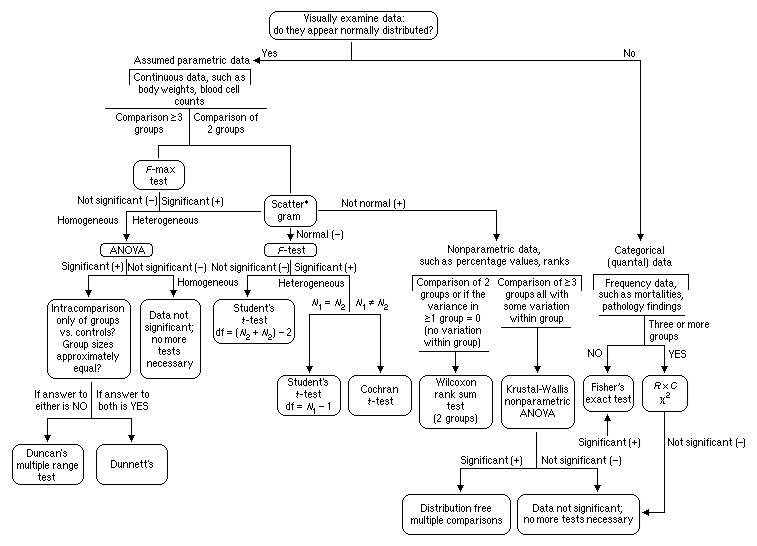
\includegraphics{images/tests_diagram.png}
\caption{}
\end{figure}

\end{frame}

\begin{frame}{Our overarching regression framework}

\[
  \begin{aligned}  
  y_{i}=a+bx_{i}+\varepsilon _{i} \\  
  \varepsilon _{i}\sim N\left( 0,\sigma^2 \right) \\  
  \end{aligned}  
\]

\begincols

\begincol

\begin{flushleft}\includegraphics{knitr_output/figures/regplot-1} \end{flushleft}

\endcol

\begincol

\textbf{Data}\\
\emph{y} = response variable\\
\emph{x} = predictor

\textbf{Parameters}\\
\emph{a} = intercept\\
\emph{b} = slope\\
\(\sigma\) = residual variation\\
\(\varepsilon\) = residuals

\endcol
\endcols

\end{frame}

\begin{frame}{Residual variation (error)}

\begincols
\begincol
\includegraphics{knitr_output/figures/small_residuals-1.pdf} \endcol

\begincol
\includegraphics{knitr_output/figures/large_residuals-1.pdf} \endcol
\endcols

\end{frame}

\begin{frame}{Residual variation}

\[
  \begin{aligned}  
  \varepsilon _{i}\sim N\left( 0,\sigma^2 \right) \\  
  \end{aligned}  
\]

\begin{center}\includegraphics{knitr_output/figures/sigmas-1} \end{center}

\end{frame}

\begin{frame}{In a Normal distribution}

\begin{figure}[htbp]
\centering
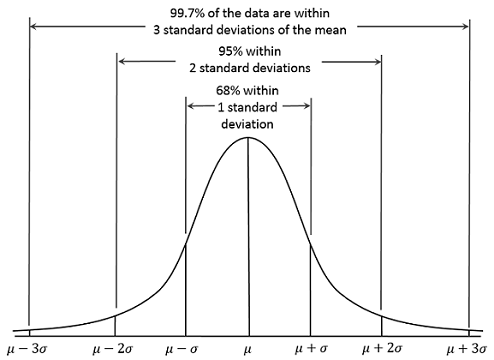
\includegraphics{images/gaussian.png}
\caption{}
\end{figure}

\end{frame}

\section{Quick refresher of linear
models}\label{quick-refresher-of-linear-models}

\begin{frame}[fragile]

\begin{itemize}[<+->]
\item
  Download datasets from \url{http://bit.ly/DEAD_datasets}
\item
  Load \texttt{iris} data into R
\item
  Q: What is the relationship between petal width and length in
  \emph{Iris setosa}?
\end{itemize}

\end{frame}

\begin{frame}[fragile]{Iris dataset}

\begin{Shaded}
\begin{Highlighting}[]
\KeywordTok{str}\NormalTok{(setosa)}
\end{Highlighting}
\end{Shaded}

\begin{verbatim}
'data.frame':   50 obs. of  5 variables:
 $ Sepal.Length: num  5.1 4.9 4.7 4.6 5 5.4 4.6 5 4.4 4.9 ...
 $ Sepal.Width : num  3.5 3 3.2 3.1 3.6 3.9 3.4 3.4 2.9 3.1 ...
 $ Petal.Length: num  1.4 1.4 1.3 1.5 1.4 1.7 1.4 1.5 1.4 1.5 ...
 $ Petal.Width : num  0.2 0.2 0.2 0.2 0.2 0.4 0.3 0.2 0.2 0.1 ...
 $ Species     : Factor w/ 3 levels "setosa","versicolor",..: 1 1 1 1 1 1 1 1 1 1 ...
\end{verbatim}

\end{frame}

\begin{frame}{Always plot your data first!}

\begin{figure}[htbp]
\centering
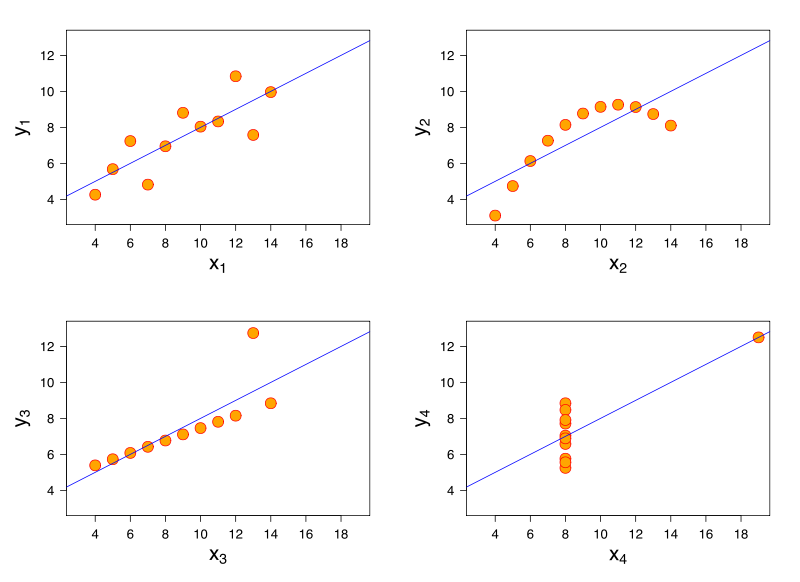
\includegraphics{images/anscombe.png}
\caption{}
\end{figure}

\end{frame}

\begin{frame}[fragile]{Exploratory Data Analysis (EDA)}

Outliers

\begin{Shaded}
\begin{Highlighting}[]
\KeywordTok{plot}\NormalTok{(setosa$Petal.Width, }\DataTypeTok{main =} \StringTok{"Petal width"}\NormalTok{)}
\end{Highlighting}
\end{Shaded}

\includegraphics{knitr_output/figures/indexplot-1.pdf}

\begin{Shaded}
\begin{Highlighting}[]
\CommentTok{#plot(setosa$Petal.Length, main = "Petal length")}
\end{Highlighting}
\end{Shaded}

\end{frame}

\begin{frame}{Outliers impact on regression}

\begin{figure}[htbp]
\centering
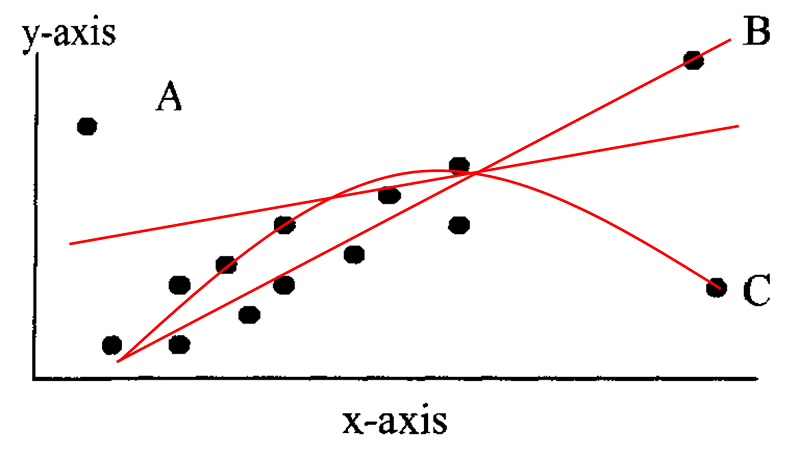
\includegraphics{images/reg_outliers.png}
\caption{}
\end{figure}

See \url{http://rpsychologist.com/d3/correlation/}

\end{frame}

\begin{frame}[fragile]{Histogram}

\begin{Shaded}
\begin{Highlighting}[]
\KeywordTok{hist}\NormalTok{(setosa$Petal.Length, }\DataTypeTok{main =} \StringTok{"Petal length"}\NormalTok{)}
\end{Highlighting}
\end{Shaded}

\includegraphics{knitr_output/figures/histog-1.pdf}

\end{frame}

\begin{frame}[fragile]{Scatterplot}

\begin{Shaded}
\begin{Highlighting}[]
\KeywordTok{plot}\NormalTok{(setosa$Petal.Width, setosa$Petal.Length, }\DataTypeTok{las =} \DecValTok{1}\NormalTok{)}
\end{Highlighting}
\end{Shaded}

\includegraphics{knitr_output/figures/scatterplot-1.pdf}

\end{frame}

\begin{frame}[fragile]{Now fit model}

Hint: \texttt{lm}

\end{frame}

\begin{frame}[fragile]{Now fit model}

Hint: \texttt{lm}

\begin{Shaded}
\begin{Highlighting}[]
\NormalTok{m1 <-}\StringTok{ }\KeywordTok{lm}\NormalTok{(Petal.Length ~}\StringTok{ }\NormalTok{Petal.Width, }\DataTypeTok{data =} \NormalTok{setosa)}
\end{Highlighting}
\end{Shaded}

\end{frame}

\begin{frame}[fragile]{What does this mean?}

\begin{verbatim}

Call:
lm(formula = Petal.Length ~ Petal.Width, data = setosa)

Residuals:
     Min       1Q   Median       3Q      Max 
-0.43686 -0.09151 -0.03686  0.09018  0.46314 

Coefficients:
            Estimate Std. Error t value Pr(>|t|)    
(Intercept)  1.32756    0.05996  22.141   <2e-16 ***
Petal.Width  0.54649    0.22439   2.435   0.0186 *  
---
Signif. codes:  0 '***' 0.001 '**' 0.01 '*' 0.05 '.' 0.1 ' ' 1

Residual standard error: 0.1655 on 48 degrees of freedom
Multiple R-squared:   0.11, Adjusted R-squared:  0.09144 
F-statistic: 5.931 on 1 and 48 DF,  p-value: 0.01864
\end{verbatim}

\end{frame}

\begin{frame}[fragile]{Retrieving model coefficients}

\begin{Shaded}
\begin{Highlighting}[]
\KeywordTok{coef}\NormalTok{(m1)}
\end{Highlighting}
\end{Shaded}

\begin{verbatim}
(Intercept) Petal.Width 
  1.3275634   0.5464903 
\end{verbatim}

\end{frame}

\begin{frame}[fragile]{Confidence intervals}

\begin{Shaded}
\begin{Highlighting}[]
\KeywordTok{confint}\NormalTok{(m1)}
\end{Highlighting}
\end{Shaded}

\begin{verbatim}
                 2.5 %    97.5 %
(Intercept) 1.20700694 1.4481199
Petal.Width 0.09531905 0.9976615
\end{verbatim}

\end{frame}

\begin{frame}[fragile]{Plot effects}

\begin{Shaded}
\begin{Highlighting}[]
\KeywordTok{library}\NormalTok{(effects)}
\KeywordTok{plot}\NormalTok{(}\KeywordTok{allEffects}\NormalTok{(m1))}
\end{Highlighting}
\end{Shaded}

\includegraphics{knitr_output/figures/unnamed-chunk-4-1.pdf}

\end{frame}

\begin{frame}[fragile]{Plot model (visreg)}

\begin{Shaded}
\begin{Highlighting}[]
\KeywordTok{library}\NormalTok{(visreg)}
\KeywordTok{visreg}\NormalTok{(m1)}
\end{Highlighting}
\end{Shaded}

\includegraphics{knitr_output/figures/visreg-1.pdf}

\end{frame}

\begin{frame}{Linear model assumptions}

\begin{itemize}[<+->]
\item
  Linearity (transformations, GAM\ldots{})
\item
  Residuals:

  \begin{itemize}[<+->]
  \tightlist
  \item
    Independent
  \item
    Equal variance
  \item
    Normal
  \end{itemize}
\item
  No measurement error in predictors
\end{itemize}

\end{frame}

\begin{frame}{Model checking: residuals}

\includegraphics{knitr_output/figures/plot_lm-1.pdf}

\end{frame}

\begin{frame}[fragile]{Are residuals normal?}

\begincols

\begincol

\begin{Shaded}
\begin{Highlighting}[]
\KeywordTok{hist}\NormalTok{(}\KeywordTok{resid}\NormalTok{(m1))}
\end{Highlighting}
\end{Shaded}

\includegraphics{knitr_output/figures/resid_hist-1.pdf} \endcol

\begincol

\begin{verbatim}
lm(formula = Petal.Length ~ Petal.Width, data = setosa)
            coef.est coef.se
(Intercept) 1.33     0.06   
Petal.Width 0.55     0.22   
---
n = 50, k = 2
residual sd = 0.17, R-Squared = 0.11
\end{verbatim}

\endcol

\endcols

SD of residuals = 0.16 coincides with estimate of \texttt{sigma}.

\end{frame}

\begin{frame}[fragile]{How good is the model in predicting petal
length?}

Observed vs Predicted values: use \texttt{fitted}.

\begin{Shaded}
\begin{Highlighting}[]
\KeywordTok{plot}\NormalTok{(setosa$Petal.Length, }\KeywordTok{fitted}\NormalTok{(m1), }\DataTypeTok{xlab =} \StringTok{"Petal length - observed"}\NormalTok{, }\DataTypeTok{ylab =} \StringTok{"Petal length - predicted"}\NormalTok{, }\DataTypeTok{las =} \DecValTok{1}\NormalTok{, }\DataTypeTok{xlim =} \KeywordTok{c}\NormalTok{(}\DecValTok{1}\NormalTok{,}\DecValTok{2}\NormalTok{), }\DataTypeTok{ylim =} \KeywordTok{c}\NormalTok{(}\DecValTok{1}\NormalTok{,}\DecValTok{2}\NormalTok{))}
\end{Highlighting}
\end{Shaded}

\includegraphics{knitr_output/figures/obs_pred-1.pdf}

Concordant with low R-squared!

\end{frame}

\begin{frame}{Using fitted model for prediction}

Q: Expected petal length if width = 0.39?

\end{frame}

\begin{frame}[fragile]{Using fitted model for prediction}

Q: Expected petal length if width = 0.39?

\begin{Shaded}
\begin{Highlighting}[]
\KeywordTok{predict}\NormalTok{(m1, }\KeywordTok{data.frame}\NormalTok{(}\DataTypeTok{Petal.Width =} \KeywordTok{c}\NormalTok{(}\FloatTok{0.39}\NormalTok{)), }\DataTypeTok{se.fit =} \OtherTok{TRUE}\NormalTok{)}
\end{Highlighting}
\end{Shaded}

\begin{verbatim}
$fit
       1 
1.540695 

$se.fit
[1] 0.03990149

$df
[1] 48

$residual.scale
[1] 0.1655341
\end{verbatim}

\end{frame}

\begin{frame}[fragile]{Important functions}

\begin{itemize}[<+->]
\item
  \texttt{plot}
\item
  \texttt{summary}
\item
  \texttt{coef}
\item
  \texttt{confint}
\item
  \texttt{fitted}
\item
  \texttt{resid}
\item
  \texttt{allEffects}
\item
  \texttt{predict}
\end{itemize}

\end{frame}

\section{Categorical predictors
(factors)}\label{categorical-predictors-factors}

\begin{frame}[fragile]{Q: Does petal length vary among \emph{Iris}
species?}

First, a plot:

\begin{Shaded}
\begin{Highlighting}[]
\KeywordTok{plot}\NormalTok{(Petal.Length ~}\StringTok{ }\NormalTok{Species, }\DataTypeTok{data =} \NormalTok{iris)}
\end{Highlighting}
\end{Shaded}

\includegraphics{knitr_output/figures/boxplot-1.pdf}

\end{frame}

\begin{frame}{Linear model with categorical predictors}

\[
  \begin{aligned} 
  y_{i}=a+bx_{i}+\varepsilon _{i} \\  
  y_{i}=a+b_{versicolor}+c_{virginica}+\varepsilon _{i} \\     
  \end{aligned} 
\]

\end{frame}

\begin{frame}[fragile]{Model}

\begin{Shaded}
\begin{Highlighting}[]
\NormalTok{m2 <-}\StringTok{ }\KeywordTok{lm}\NormalTok{(Petal.Length ~}\StringTok{ }\NormalTok{Species, }\DataTypeTok{data =} \NormalTok{iris)}
\end{Highlighting}
\end{Shaded}

\begin{verbatim}

Call:
lm(formula = Petal.Length ~ Species, data = iris)

Residuals:
   Min     1Q Median     3Q    Max 
-1.260 -0.258  0.038  0.240  1.348 

Coefficients:
                  Estimate Std. Error t value Pr(>|t|)    
(Intercept)        1.46200    0.06086   24.02   <2e-16 ***
Speciesversicolor  2.79800    0.08607   32.51   <2e-16 ***
Speciesvirginica   4.09000    0.08607   47.52   <2e-16 ***
---
Signif. codes:  0 '***' 0.001 '**' 0.01 '*' 0.05 '.' 0.1 ' ' 1

Residual standard error: 0.4303 on 147 degrees of freedom
Multiple R-squared:  0.9414,    Adjusted R-squared:  0.9406 
F-statistic:  1180 on 2 and 147 DF,  p-value: < 2.2e-16
\end{verbatim}

\end{frame}

\begin{frame}[fragile]{Alternatively, no intercept}

\begin{Shaded}
\begin{Highlighting}[]
\NormalTok{m3 <-}\StringTok{ }\KeywordTok{lm}\NormalTok{(Petal.Length ~}\StringTok{ }\NormalTok{Species -}\StringTok{ }\DecValTok{1}\NormalTok{, }\DataTypeTok{data =} \NormalTok{iris)}
\end{Highlighting}
\end{Shaded}

\begin{verbatim}

Call:
lm(formula = Petal.Length ~ Species - 1, data = iris)

Residuals:
   Min     1Q Median     3Q    Max 
-1.260 -0.258  0.038  0.240  1.348 

Coefficients:
                  Estimate Std. Error t value Pr(>|t|)    
Speciessetosa      1.46200    0.06086   24.02   <2e-16 ***
Speciesversicolor  4.26000    0.06086   70.00   <2e-16 ***
Speciesvirginica   5.55200    0.06086   91.23   <2e-16 ***
---
Signif. codes:  0 '***' 0.001 '**' 0.01 '*' 0.05 '.' 0.1 ' ' 1

Residual standard error: 0.4303 on 147 degrees of freedom
Multiple R-squared:  0.9895,    Adjusted R-squared:  0.9892 
F-statistic:  4600 on 3 and 147 DF,  p-value: < 2.2e-16
\end{verbatim}

\end{frame}

\begin{frame}[fragile]{Petal length differences across 3 \emph{Iris}
species}

\begin{Shaded}
\begin{Highlighting}[]
\KeywordTok{visreg}\NormalTok{(m3)}
\end{Highlighting}
\end{Shaded}

\includegraphics{knitr_output/figures/iris_plot-1.pdf}

\end{frame}

\begin{frame}[fragile]{Are differences statistically significant?}

Compare CIs

\begin{Shaded}
\begin{Highlighting}[]
\KeywordTok{summary}\NormalTok{(}\KeywordTok{allEffects}\NormalTok{(m3))}
\end{Highlighting}
\end{Shaded}

\begin{verbatim}
 model: Petal.Length ~ Species - 1

 Species effect
Species
    setosa versicolor  virginica 
     1.462      4.260      5.552 

 Lower 95 Percent Confidence Limits
Species
    setosa versicolor  virginica 
  1.341729   4.139729   5.431729 

 Upper 95 Percent Confidence Limits
Species
    setosa versicolor  virginica 
  1.582271   4.380271   5.672271 
\end{verbatim}

\end{frame}

\begin{frame}[fragile]{Plotting effects}

\begin{Shaded}
\begin{Highlighting}[]
\KeywordTok{plot}\NormalTok{(}\KeywordTok{allEffects}\NormalTok{(m3))}
\end{Highlighting}
\end{Shaded}

\includegraphics{knitr_output/figures/unnamed-chunk-7-1.pdf}

\end{frame}

\section{Combining continuous and categorical
predictors}\label{combining-continuous-and-categorical-predictors}

\begin{frame}{Predicting \emph{Iris} petal length according to species
and petal width}

\[
  \begin{aligned} 
  y_{i}=a+bx_{i}+\varepsilon _{i} \\  
  y_{i}=a+b_{versicolor}+c_{virginica}+\varepsilon _{i} \\   
  y_{i}=a+b_{versicolor}+c_{virginica}+ d \cdot PetalWidth_{i} + \varepsilon _{i} \\   
  \end{aligned} 
\]

\end{frame}

\begin{frame}[fragile]{Predicting \emph{Iris} petal length according to
species and petal width}

\begin{verbatim}

Call:
lm(formula = Petal.Length ~ Species + Petal.Width, data = iris)

Residuals:
     Min       1Q   Median       3Q      Max 
-1.02977 -0.22241 -0.01514  0.18180  1.17449 

Coefficients:
                  Estimate Std. Error t value Pr(>|t|)    
(Intercept)        1.21140    0.06524  18.568  < 2e-16 ***
Speciesversicolor  1.69779    0.18095   9.383  < 2e-16 ***
Speciesvirginica   2.27669    0.28132   8.093 2.08e-13 ***
Petal.Width        1.01871    0.15224   6.691 4.41e-10 ***
---
Signif. codes:  0 '***' 0.001 '**' 0.01 '*' 0.05 '.' 0.1 ' ' 1

Residual standard error: 0.3777 on 146 degrees of freedom
Multiple R-squared:  0.9551,    Adjusted R-squared:  0.9542 
F-statistic:  1036 on 3 and 146 DF,  p-value: < 2.2e-16
\end{verbatim}

\end{frame}

\section{Generalised Linear Models
(GLMs)}\label{generalised-linear-models-glms}

\begin{frame}[fragile]{Q: Survival of passengers on the Titanic
\textasciitilde{} Class}

Read \texttt{titanic\_long.csv} dataset.

\begin{verbatim}
  class   age  sex survived
1 first adult male        1
2 first adult male        1
3 first adult male        1
4 first adult male        1
5 first adult male        1
6 first adult male        1
\end{verbatim}

\end{frame}

\begin{frame}[fragile]{Let's fit linear model:}

\begin{Shaded}
\begin{Highlighting}[]
\NormalTok{m5 <-}\StringTok{ }\KeywordTok{lm}\NormalTok{(survived ~}\StringTok{ }\NormalTok{class, }\DataTypeTok{data =} \NormalTok{titanic)}
\end{Highlighting}
\end{Shaded}

\includegraphics{knitr_output/figures/titanic_lm-1.pdf}

\end{frame}

\begin{frame}{Weird residuals!}

\includegraphics{knitr_output/figures/titanic_lm_resid-1.pdf}

\end{frame}

\begin{frame}{What if your residuals are clearly non-normal? \textbar{}
And variance not constant (heteroscedasticity)?}

\begin{itemize}[<+->]
\tightlist
\item
  Binary variables (0/1)
\item
  Counts (0, 1, 2, 3, \ldots{})
\end{itemize}

\end{frame}

\begin{frame}[fragile]{Generalised Linear Models}

\begin{enumerate}[<+->]
\def\labelenumi{\arabic{enumi}.}
\item
  \textbf{Response variable} - distribution \texttt{family}

  \begin{itemize}[<+->]
  \tightlist
  \item
    Bernouilli - Binomial
  \item
    Poisson
  \item
    Gamma
  \item
    etc
  \end{itemize}
\item
  \textbf{Predictors} (continuous or categorical)
\item
  \textbf{Link function}

  \begin{itemize}[<+->]
  \tightlist
  \item
    Gaussian: identity
  \item
    Binomial: logit, probit
  \item
    Poisson: log\ldots{}
  \item
    See
    \href{http://www.rdocumentation.org/packages/stats/functions/family}{\texttt{family}}.
  \end{itemize}
\end{enumerate}

\end{frame}

\begin{frame}{The modelling process}

\begin{figure}[htbp]
\centering
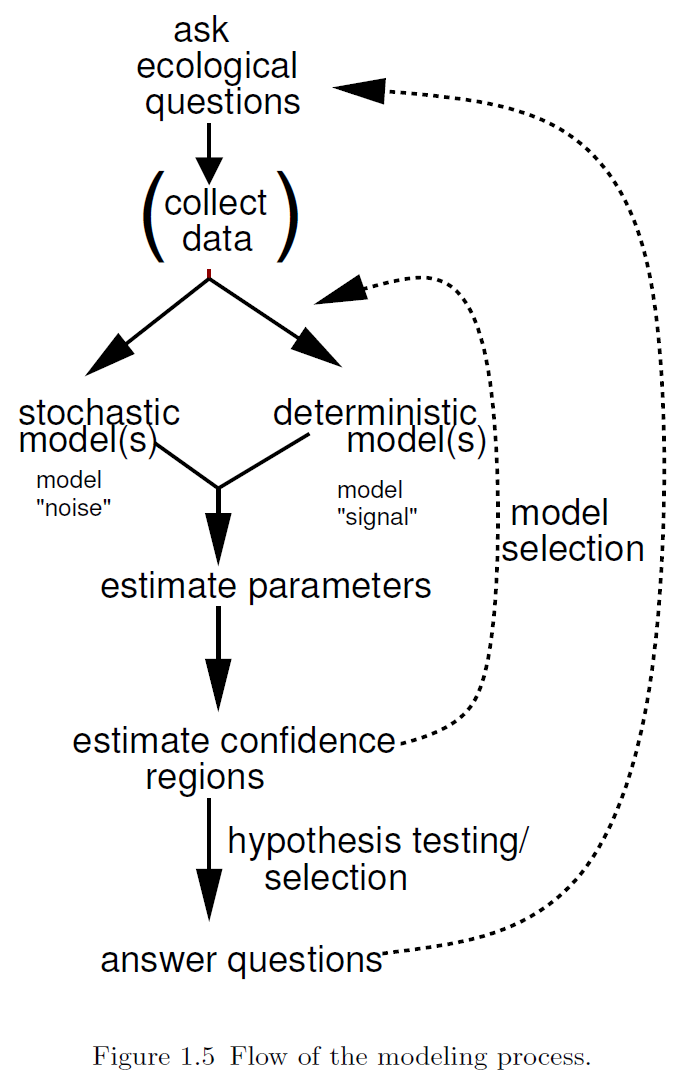
\includegraphics{images/modeling_process.png}
\caption{}
\end{figure}

Bolker 2008

\end{frame}

\begin{frame}[fragile]{Bernouilli - Binomial distribution (Logistic
regression)}

\begin{itemize}[<+->]
\tightlist
\item
  Response variable: Yes/No (e.g.~survival, sex, presence/absence)
\item
  Link function: \texttt{logit} (others possible, see \texttt{family}).
\end{itemize}

\[
  \begin{aligned} 
  logit(p) = \ln \left( \dfrac {p} {1-p}\right) \\ 
  \end{aligned} 
\]

Then

\[
  \begin{aligned} 
  Pr(alive) = a + bx \\  
  logit(Pr(alive)) = a + bx \\  
  Pr(alive) = invlogit(a + bx) = \dfrac {e^{a+bx}} {1+e^{a+bx}} \\  
  \end{aligned} 
\]

\end{frame}

\begin{frame}{Back to survival of Titanic passengers}

How many passengers travelled in each class?

\end{frame}

\begin{frame}[fragile]{Back to survival of Titanic passengers}

How many passengers travelled in each class?

\begin{Shaded}
\begin{Highlighting}[]
\KeywordTok{tapply}\NormalTok{(titanic$survived, titanic$class, length)}
\end{Highlighting}
\end{Shaded}

\begin{verbatim}
  crew  first second  third 
   885    325    285    706 
\end{verbatim}

\end{frame}

\begin{frame}[fragile]{Back to survival of Titanic passengers}

How many passengers travelled in each class?

\begin{Shaded}
\begin{Highlighting}[]
\KeywordTok{tapply}\NormalTok{(titanic$survived, titanic$class, length)}
\end{Highlighting}
\end{Shaded}

\begin{verbatim}
  crew  first second  third 
   885    325    285    706 
\end{verbatim}

How many survived?

\end{frame}

\begin{frame}[fragile]{Back to survival of Titanic passengers}

How many passengers travelled in each class?

\begin{Shaded}
\begin{Highlighting}[]
\KeywordTok{tapply}\NormalTok{(titanic$survived, titanic$class, length)}
\end{Highlighting}
\end{Shaded}

\begin{verbatim}
  crew  first second  third 
   885    325    285    706 
\end{verbatim}

How many survived?

\begin{Shaded}
\begin{Highlighting}[]
\KeywordTok{tapply}\NormalTok{(titanic$survived, titanic$class, sum)}
\end{Highlighting}
\end{Shaded}

\begin{verbatim}
  crew  first second  third 
   212    203    118    178 
\end{verbatim}

\end{frame}

\begin{frame}[fragile]{Back to survival of Titanic passengers}

How many passengers travelled in each class?

\begin{Shaded}
\begin{Highlighting}[]
\KeywordTok{tapply}\NormalTok{(titanic$survived, titanic$class, length)}
\end{Highlighting}
\end{Shaded}

\begin{verbatim}
  crew  first second  third 
   885    325    285    706 
\end{verbatim}

How many survived?

\begin{Shaded}
\begin{Highlighting}[]
\KeywordTok{tapply}\NormalTok{(titanic$survived, titanic$class, sum)}
\end{Highlighting}
\end{Shaded}

\begin{verbatim}
  crew  first second  third 
   212    203    118    178 
\end{verbatim}

What proportion survived in each class?

\begin{Shaded}
\begin{Highlighting}[]
\KeywordTok{as.numeric}\NormalTok{(}\KeywordTok{tapply}\NormalTok{(titanic$survived, titanic$class, mean))}
\end{Highlighting}
\end{Shaded}

\begin{verbatim}
[1] 0.2395480 0.6246154 0.4140351 0.2521246
\end{verbatim}

\end{frame}

\begin{frame}[fragile]{Back to survival of Titanic passengers (dplyr)}

Passenger survival according to class

\begin{Shaded}
\begin{Highlighting}[]
\KeywordTok{library}\NormalTok{(dplyr)}
\NormalTok{titanic %>%}
\StringTok{  }\KeywordTok{group_by}\NormalTok{(class, survived) %>%}
\StringTok{  }\KeywordTok{summarise}\NormalTok{(}\DataTypeTok{count =} \KeywordTok{n}\NormalTok{())}
\end{Highlighting}
\end{Shaded}

\begin{verbatim}
Source: local data frame [8 x 3]
Groups: class [?]

   class survived count
  <fctr>    <int> <int>
1   crew        0   673
2   crew        1   212
3  first        0   122
4  first        1   203
5 second        0   167
6 second        1   118
7  third        0   528
8  third        1   178
\end{verbatim}

Or
\texttt{summarise(group\_by(titanic,\ class,\ survived),\ count\ =\ n())}

\end{frame}

\begin{frame}[fragile]{Or graphically\ldots{}}

\begin{Shaded}
\begin{Highlighting}[]
\KeywordTok{plot}\NormalTok{(}\KeywordTok{factor}\NormalTok{(survived) ~}\StringTok{ }\NormalTok{class, }\DataTypeTok{data =} \NormalTok{titanic)}
\end{Highlighting}
\end{Shaded}

\includegraphics{knitr_output/figures/titanic_eda-1.pdf}

\end{frame}

\begin{frame}[fragile]{Fitting GLMs in R: \texttt{glm}}

\begin{Shaded}
\begin{Highlighting}[]
\NormalTok{tit.glm <-}\StringTok{ }\KeywordTok{glm}\NormalTok{(survived ~}\StringTok{ }\NormalTok{class, }\DataTypeTok{data=}\NormalTok{titanic, }\DataTypeTok{family=}\NormalTok{binomial)}
\end{Highlighting}
\end{Shaded}

\begin{verbatim}

Call:
glm(formula = survived ~ class, family = binomial, data = titanic)

Deviance Residuals: 
    Min       1Q   Median       3Q      Max  
-1.3999  -0.7623  -0.7401   0.9702   1.6906  

Coefficients:
            Estimate Std. Error z value Pr(>|z|)    
(Intercept) -1.15516    0.07876 -14.667  < 2e-16 ***
classfirst   1.66434    0.13902  11.972  < 2e-16 ***
classsecond  0.80785    0.14375   5.620 1.91e-08 ***
classthird   0.06785    0.11711   0.579    0.562    
---
Signif. codes:  0 '***' 0.001 '**' 0.01 '*' 0.05 '.' 0.1 ' ' 1

(Dispersion parameter for binomial family taken to be 1)

    Null deviance: 2769.5  on 2200  degrees of freedom
Residual deviance: 2588.6  on 2197  degrees of freedom
AIC: 2596.6

Number of Fisher Scoring iterations: 4
\end{verbatim}

These estimates are in logit scale!

\end{frame}

\begin{frame}[fragile]{Interpreting logistic regression output}

Parameter estimates (logit-scale)

\begin{verbatim}
(Intercept)  classfirst classsecond  classthird 
-1.15515905  1.66434399  0.80784987  0.06784632 
\end{verbatim}

\textbf{We need to back-transform}: apply \emph{inverse logit}\\
Crew probability of survival:

\begin{Shaded}
\begin{Highlighting}[]
\KeywordTok{plogis}\NormalTok{(}\KeywordTok{coef}\NormalTok{(tit.glm)[}\DecValTok{1}\NormalTok{])}
\end{Highlighting}
\end{Shaded}

\begin{verbatim}
(Intercept) 
   0.239548 
\end{verbatim}

Looking at the data, the proportion of crew who survived is

\begin{verbatim}
[1] 0.239548
\end{verbatim}

\end{frame}

\begin{frame}[fragile]{Q: Probability of survival for 1st class
passengers?}

\begin{Shaded}
\begin{Highlighting}[]
\KeywordTok{plogis}\NormalTok{(}\KeywordTok{coef}\NormalTok{(tit.glm)[}\DecValTok{1}\NormalTok{] +}\StringTok{ }\KeywordTok{coef}\NormalTok{(tit.glm)[}\DecValTok{2}\NormalTok{])}
\end{Highlighting}
\end{Shaded}

\begin{verbatim}
(Intercept) 
  0.6246154 
\end{verbatim}

Needs to add intercept (baseline) to the parameter estimate. Again this
value matches the data:

\begin{Shaded}
\begin{Highlighting}[]
\KeywordTok{sum}\NormalTok{(titanic$survived[titanic$class ==}\StringTok{ "first"}\NormalTok{]) /}\StringTok{   }
\StringTok{  }\KeywordTok{nrow}\NormalTok{(titanic[titanic$class ==}\StringTok{ "first"}\NormalTok{, ])}
\end{Highlighting}
\end{Shaded}

\begin{verbatim}
[1] 0.6246154
\end{verbatim}

\end{frame}

\begin{frame}[fragile]{Model interpretation using \texttt{effects}
package}

\begin{Shaded}
\begin{Highlighting}[]
\KeywordTok{library}\NormalTok{(effects)}
\KeywordTok{allEffects}\NormalTok{(tit.glm)}
\end{Highlighting}
\end{Shaded}

\begin{verbatim}
 model: survived ~ class

 class effect
class
     crew     first    second     third 
0.2395480 0.6246154 0.4140351 0.2521246 
\end{verbatim}

\end{frame}

\begin{frame}[fragile]{Effects plot}

\begin{Shaded}
\begin{Highlighting}[]
\KeywordTok{plot}\NormalTok{(}\KeywordTok{allEffects}\NormalTok{(tit.glm))}
\end{Highlighting}
\end{Shaded}

\includegraphics{knitr_output/figures/effects_plot-1.pdf}

\end{frame}

\begin{frame}{Logistic regression: model checking}

\includegraphics{knitr_output/figures/tit_glm_check-1.pdf}

Not very useful.

\end{frame}

\begin{frame}[fragile]{Binned residual plots for logistic regression}

\begin{Shaded}
\begin{Highlighting}[]
\NormalTok{predvals <-}\StringTok{ }\KeywordTok{predict}\NormalTok{(tit.glm, }\DataTypeTok{type=}\StringTok{"response"}\NormalTok{)}
\NormalTok{arm::}\KeywordTok{binnedplot}\NormalTok{(predvals, titanic$survived -}\StringTok{ }\NormalTok{predvals)}
\end{Highlighting}
\end{Shaded}

\includegraphics{knitr_output/figures/binnedplot-1.pdf}

\end{frame}

\begin{frame}[fragile]{Residual diagnostics with DHARMa}

\begin{Shaded}
\begin{Highlighting}[]
\KeywordTok{library}\NormalTok{(DHARMa)}
\KeywordTok{simulateResiduals}\NormalTok{(tit.glm, }\DataTypeTok{plot =} \OtherTok{TRUE}\NormalTok{)}
\end{Highlighting}
\end{Shaded}

\includegraphics{knitr_output/figures/unnamed-chunk-16-1.pdf}

\begin{verbatim}
Object of Class DHARMa with simulated residuals based on 250 simulations with refit = FALSE . See ?DHARMa::simulateResiduals for help. 
 
Scaled residual values: 0.972 0.552 0.8 0.74 0.42 0.888 0.536 0.956 0.904 0.864 0.832 0.84 0.636 0.496 0.772 0.928 0.42 0.504 1 0.504 ...
\end{verbatim}

See
\url{https://cran.r-project.org/web/packages/DHARMa/vignettes/DHARMa.html}

\end{frame}

\begin{frame}[fragile]{Recapitulating}

\begin{enumerate}[<+->]
\def\labelenumi{\arabic{enumi}.}
\item
  Import data: \texttt{read.table} or \texttt{read.csv}
\item
  Check data: \texttt{summary}
\item
  Plot data: \texttt{plot}
\item
  Fit model: \texttt{glm}. Don't forget to specify \texttt{family}!
\item
  Examine models: \texttt{summary}
\item
  Use \texttt{plogis} to apply back-transformation (\emph{invlogit}) to
  parameter estimates (\texttt{coef}). Alternatively, use
  \texttt{allEffects} from \texttt{effects} package.
\item
  Plot model: \texttt{plot(allEffects(model))}. Or use \texttt{visreg}.
\item
  Examine residuals: use \texttt{arm::binnedplot} or
  \texttt{DHARMa::simulateResiduals}.
\end{enumerate}

\end{frame}

\section{Q: Did men have higher survival than
women?}\label{q-did-men-have-higher-survival-than-women}

\begin{frame}[fragile]{Plot first}

\begin{Shaded}
\begin{Highlighting}[]
\KeywordTok{plot}\NormalTok{(}\KeywordTok{factor}\NormalTok{(survived) ~}\StringTok{ }\NormalTok{sex, }\DataTypeTok{data =} \NormalTok{titanic)}
\end{Highlighting}
\end{Shaded}

\includegraphics{knitr_output/figures/tit_sex_eda-1.pdf}

\end{frame}

\begin{frame}[fragile]{Fit model}

\begin{Shaded}
\begin{Highlighting}[]
\NormalTok{tit.sex <-}\StringTok{ }\KeywordTok{glm}\NormalTok{(survived ~}\StringTok{ }\NormalTok{sex, }\DataTypeTok{data =} \NormalTok{titanic, }\DataTypeTok{family =} \NormalTok{binomial)}
\end{Highlighting}
\end{Shaded}

\begin{verbatim}

Call:
glm(formula = survived ~ sex, family = binomial, data = titanic)

Deviance Residuals: 
    Min       1Q   Median       3Q      Max  
-1.6226  -0.6903  -0.6903   0.7901   1.7613  

Coefficients:
            Estimate Std. Error z value Pr(>|z|)    
(Intercept)   1.0044     0.1041   9.645   <2e-16 ***
sexmale      -2.3172     0.1196 -19.376   <2e-16 ***
---
Signif. codes:  0 '***' 0.001 '**' 0.01 '*' 0.05 '.' 0.1 ' ' 1

(Dispersion parameter for binomial family taken to be 1)

    Null deviance: 2769.5  on 2200  degrees of freedom
Residual deviance: 2335.0  on 2199  degrees of freedom
AIC: 2339

Number of Fisher Scoring iterations: 4
\end{verbatim}

\end{frame}

\begin{frame}[fragile]{Effects}

\begincols
\begincol

\begin{verbatim}
 model: survived ~ sex

 sex effect
sex
   female      male 
0.7319149 0.2120162 
\end{verbatim}

\endcol

\begincol
\includegraphics{knitr_output/figures/tit_sex_effects2-1.pdf} \endcol
\endcols

\end{frame}

\section{Q: Did women have higher survival because they travelled more
in first
class?}\label{q-did-women-have-higher-survival-because-they-travelled-more-in-first-class}

\begin{frame}[fragile]{Let's look at the data}

\texttt{tapply}

\begin{Shaded}
\begin{Highlighting}[]
\KeywordTok{tapply}\NormalTok{(titanic$survived, }\KeywordTok{list}\NormalTok{(titanic$class, titanic$sex), sum)}
\end{Highlighting}
\end{Shaded}

\begin{verbatim}
       female male
crew       20  192
first     141   62
second     93   25
third      90   88
\end{verbatim}

Mmmm\ldots{}

\end{frame}

\begin{frame}[fragile]{Fit model with both factors (interactions)}

\begin{Shaded}
\begin{Highlighting}[]
\NormalTok{tit.sex.class <-}\StringTok{ }\KeywordTok{glm}\NormalTok{(survived ~}\StringTok{ }\NormalTok{class *}\StringTok{ }\NormalTok{sex, }\DataTypeTok{data =} \NormalTok{titanic, }\DataTypeTok{family =} \NormalTok{binomial)}
\end{Highlighting}
\end{Shaded}

\begin{verbatim}
glm(formula = survived ~ class * sex, family = binomial, data = titanic)
                    coef.est coef.se
(Intercept)          1.90     0.62  
classfirst           1.67     0.80  
classsecond          0.07     0.69  
classthird          -2.06     0.64  
sexmale             -3.15     0.62  
classfirst:sexmale  -1.06     0.82  
classsecond:sexmale -0.64     0.72  
classthird:sexmale   1.74     0.65  
---
  n = 2201, k = 8
  residual deviance = 2163.7, null deviance = 2769.5 (difference = 605.7)
\end{verbatim}

\end{frame}

\begin{frame}[fragile]{Effects}

\begincols
\begincol

\begin{verbatim}
 model: survived ~ class * sex

 class*sex effect
        sex
class       female      male
  crew   0.8695652 0.2227378
  first  0.9724138 0.3444444
  second 0.8773585 0.1396648
  third  0.4591837 0.1725490
\end{verbatim}

\endcol

\begincol
\includegraphics{knitr_output/figures/tit_sex_class_effects2-1.pdf}
\endcol
\endcols

So, women had higher probability of survival than men, even within the
same class.

\end{frame}

\section{Logistic regression for proportion
data}\label{logistic-regression-for-proportion-data}

\begin{frame}[fragile]{Read Titanic data in different format}

Read \texttt{Titanic\_prop.csv} data.

\begin{verbatim}
       X          Class       Sex       Age          No        
 Min.   : 1.00   1st :4   Female:8   Adult:8   Min.   :  0.00  
 1st Qu.: 4.75   2nd :4   Male  :8   Child:8   1st Qu.:  0.00  
 Median : 8.50   3rd :4                        Median :  8.50  
 Mean   : 8.50   Crew:4                        Mean   : 93.12  
 3rd Qu.:12.25                                 3rd Qu.: 96.25  
 Max.   :16.00                                 Max.   :670.00  
      Yes        
 Min.   :  0.00  
 1st Qu.:  9.50  
 Median : 14.00  
 Mean   : 44.44  
 3rd Qu.: 75.25  
 Max.   :192.00  
\end{verbatim}

These are the same data, but summarized (see \texttt{Freq} variable).

\end{frame}

\begin{frame}[fragile]{Use cbind(n.success, n.failures) as response}

\begin{Shaded}
\begin{Highlighting}[]
\NormalTok{prop.glm <-}\StringTok{ }\KeywordTok{glm}\NormalTok{(}\KeywordTok{cbind}\NormalTok{(Yes, No) ~}\StringTok{ }\NormalTok{Class, }\DataTypeTok{data =} \NormalTok{tit.prop, }\DataTypeTok{family =} \NormalTok{binomial)}
\end{Highlighting}
\end{Shaded}

\begin{verbatim}

Call:
glm(formula = cbind(Yes, No) ~ Class, family = binomial, data = tit.prop)

Deviance Residuals: 
    Min       1Q   Median       3Q      Max  
-9.6404  -0.2915   1.5698   5.0366  10.1516  

Coefficients:
            Estimate Std. Error z value Pr(>|z|)    
(Intercept)   0.5092     0.1146   4.445 8.79e-06 ***
Class2nd     -0.8565     0.1661  -5.157 2.51e-07 ***
Class3rd     -1.5965     0.1436 -11.114  < 2e-16 ***
ClassCrew    -1.6643     0.1390 -11.972  < 2e-16 ***
---
Signif. codes:  0 '***' 0.001 '**' 0.01 '*' 0.05 '.' 0.1 ' ' 1

(Dispersion parameter for binomial family taken to be 1)

    Null deviance: 671.96  on 13  degrees of freedom
Residual deviance: 491.06  on 10  degrees of freedom
AIC: 545.68

Number of Fisher Scoring iterations: 4
\end{verbatim}

\end{frame}

\begin{frame}[fragile]{Effects}

\begin{verbatim}
 model: cbind(Yes, No) ~ Class

 Class effect
Class
      1st       2nd       3rd      Crew 
0.6246154 0.4140351 0.2521246 0.2395480 
\end{verbatim}

Compare with former model based on raw data:

\begin{verbatim}
 model: survived ~ class

 class effect
class
     crew     first    second     third 
0.2395480 0.6246154 0.4140351 0.2521246 
\end{verbatim}

Same results!

\end{frame}

\section{Logistic regression with continuous
predictors}\label{logistic-regression-with-continuous-predictors}

\begin{frame}[fragile]

Example dataset:
\href{http://vincentarelbundock.github.io/Rdatasets/doc/car/UN.html}{GDP
and infant mortality}

Read \texttt{UN\_GDP\_infantmortality.csv}.

\begin{verbatim}
           country      mortality           gdp       
 Afghanistan   :  1   Min.   :  2.00   Min.   :   36  
 Albania       :  1   1st Qu.: 12.00   1st Qu.:  442  
 Algeria       :  1   Median : 30.00   Median : 1779  
 American.Samoa:  1   Mean   : 43.48   Mean   : 6262  
 Andorra       :  1   3rd Qu.: 66.00   3rd Qu.: 7272  
 Angola        :  1   Max.   :169.00   Max.   :42416  
 (Other)       :201   NA's   :6        NA's   :10     
\end{verbatim}

\end{frame}

\begin{frame}[fragile]{EDA}

\begin{Shaded}
\begin{Highlighting}[]
\KeywordTok{plot}\NormalTok{(mortality ~}\StringTok{ }\NormalTok{gdp, }\DataTypeTok{data =} \NormalTok{gdp, }\DataTypeTok{main =} \StringTok{"Infant mortality (per 1000 births)"}\NormalTok{)}
\end{Highlighting}
\end{Shaded}

\includegraphics{knitr_output/figures/gdp_eda-1.pdf}

\end{frame}

\begin{frame}[fragile]{Fit model}

\begin{Shaded}
\begin{Highlighting}[]
\NormalTok{gdp.glm <-}\StringTok{ }\KeywordTok{glm}\NormalTok{(}\KeywordTok{cbind}\NormalTok{(mortality, }\DecValTok{1000} \NormalTok{-}\StringTok{ }\NormalTok{mortality) ~}\StringTok{ }\NormalTok{gdp, }
               \DataTypeTok{data =} \NormalTok{gdp, }\DataTypeTok{family =} \NormalTok{binomial)}
\end{Highlighting}
\end{Shaded}

\begin{verbatim}

Call:
glm(formula = cbind(mortality, 1000 - mortality) ~ gdp, family = binomial, 
    data = gdp)

Deviance Residuals: 
    Min       1Q   Median       3Q      Max  
-9.2230  -3.5163  -0.5697   2.4284  13.5849  

Coefficients:
              Estimate Std. Error z value Pr(>|z|)    
(Intercept) -2.657e+00  1.311e-02 -202.76   <2e-16 ***
gdp         -1.279e-04  3.458e-06  -36.98   <2e-16 ***
---
Signif. codes:  0 '***' 0.001 '**' 0.01 '*' 0.05 '.' 0.1 ' ' 1

(Dispersion parameter for binomial family taken to be 1)

    Null deviance: 6430.2  on 192  degrees of freedom
Residual deviance: 3530.2  on 191  degrees of freedom
  (14 observations deleted due to missingness)
AIC: 4525.8

Number of Fisher Scoring iterations: 5
\end{verbatim}

\end{frame}

\begin{frame}[fragile]{Effects}

\begin{Shaded}
\begin{Highlighting}[]
\KeywordTok{allEffects}\NormalTok{(gdp.glm)}
\end{Highlighting}
\end{Shaded}

\begin{verbatim}
 model: cbind(mortality, 1000 - mortality) ~ gdp

 gdp effect
gdp
       10000        20000        30000        40000 
0.0191438829 0.0054028095 0.0015096074 0.0004206154 
\end{verbatim}

\end{frame}

\begin{frame}[fragile]{Effects plot}

\begin{Shaded}
\begin{Highlighting}[]
\KeywordTok{plot}\NormalTok{(}\KeywordTok{allEffects}\NormalTok{(gdp.glm))}
\end{Highlighting}
\end{Shaded}

\includegraphics{knitr_output/figures/gdp_effectsplot-1.pdf}

\end{frame}

\begin{frame}[fragile]{Plot model and data}

\begin{Shaded}
\begin{Highlighting}[]
\KeywordTok{plot}\NormalTok{(mortality/}\DecValTok{1000} \NormalTok{~}\StringTok{ }\NormalTok{gdp, }\DataTypeTok{data =} \NormalTok{gdp, }\DataTypeTok{main =} \StringTok{"Infant mortality rate"}\NormalTok{)}
\KeywordTok{curve}\NormalTok{(}\KeywordTok{plogis}\NormalTok{(}\KeywordTok{coef}\NormalTok{(gdp.glm)[}\DecValTok{1}\NormalTok{] +}\StringTok{ }\KeywordTok{coef}\NormalTok{(gdp.glm)[}\DecValTok{2}\NormalTok{]*x), }\DataTypeTok{from =} \DecValTok{0}\NormalTok{, }\DataTypeTok{to =} \DecValTok{40000}\NormalTok{, }\DataTypeTok{add =} \OtherTok{TRUE}\NormalTok{, }\DataTypeTok{lwd=}\DecValTok{3}\NormalTok{, }\DataTypeTok{col=}\StringTok{"red"}\NormalTok{)}
\end{Highlighting}
\end{Shaded}

\includegraphics{knitr_output/figures/logistic_plot-1.pdf}

\end{frame}

\begin{frame}[fragile]{Plot model using visreg:}

\begin{Shaded}
\begin{Highlighting}[]
\KeywordTok{visreg}\NormalTok{(gdp.glm, }\DataTypeTok{scale =} \StringTok{"response"}\NormalTok{)}
\KeywordTok{points}\NormalTok{(mortality/}\DecValTok{1000} \NormalTok{~}\StringTok{ }\NormalTok{gdp, }\DataTypeTok{data =} \NormalTok{gdp)}
\end{Highlighting}
\end{Shaded}

\includegraphics{knitr_output/figures/gdp_visreg-1.pdf}

\end{frame}

\begin{frame}[fragile]{Residuals diagnostics with DHARMa}

\begin{Shaded}
\begin{Highlighting}[]
\KeywordTok{simulateResiduals}\NormalTok{(gdp.glm, }\DataTypeTok{plot =} \OtherTok{TRUE}\NormalTok{)}
\end{Highlighting}
\end{Shaded}

\includegraphics{knitr_output/figures/unnamed-chunk-17-1.pdf}

\begin{verbatim}
Object of Class DHARMa with simulated residuals based on 250 simulations with refit = FALSE . See ?DHARMa::simulateResiduals for help. 
 
Scaled residual values: 1 0 0.064 1 0.228 0.372 0 0.6 1 0 0.488 0.236 0.98 0 0 0.988 0 1 1 0.812 ...
\end{verbatim}

\end{frame}

\section{Overdispersion}\label{overdispersion}

\begin{frame}[fragile]{Testing for overdispersion (DHARMa)}

\begin{Shaded}
\begin{Highlighting}[]
\NormalTok{simres <-}\StringTok{ }\KeywordTok{simulateResiduals}\NormalTok{(gdp.glm, }\DataTypeTok{refit =} \OtherTok{TRUE}\NormalTok{)}
\KeywordTok{testOverdispersion}\NormalTok{(simres)}
\end{Highlighting}
\end{Shaded}

\begin{verbatim}

    Overdispersion test via comparison to simulation under H0

data:  simres
dispersion = 20.571, p-value < 2.2e-16
alternative hypothesis: overdispersion
\end{verbatim}

\end{frame}

\begin{frame}[fragile]{Overdispersion in logistic regression with
proportion data}

\begin{Shaded}
\begin{Highlighting}[]
\NormalTok{gdp.overdisp <-}\StringTok{ }\KeywordTok{glm}\NormalTok{(}\KeywordTok{cbind}\NormalTok{(mortality, }\DecValTok{1000} \NormalTok{-}\StringTok{ }\NormalTok{mortality) ~}\StringTok{ }\NormalTok{gdp, }
               \DataTypeTok{data =} \NormalTok{gdp, }\DataTypeTok{family =} \NormalTok{quasibinomial)}
\end{Highlighting}
\end{Shaded}

\begin{verbatim}

Call:
glm(formula = cbind(mortality, 1000 - mortality) ~ gdp, family = quasibinomial, 
    data = gdp)

Deviance Residuals: 
    Min       1Q   Median       3Q      Max  
-9.2230  -3.5163  -0.5697   2.4284  13.5849  

Coefficients:
              Estimate Std. Error t value Pr(>|t|)    
(Intercept) -2.657e+00  5.977e-02 -44.465  < 2e-16 ***
gdp         -1.279e-04  1.577e-05  -8.111 5.96e-14 ***
---
Signif. codes:  0 '***' 0.001 '**' 0.01 '*' 0.05 '.' 0.1 ' ' 1

(Dispersion parameter for quasibinomial family taken to be 20.7947)

    Null deviance: 6430.2  on 192  degrees of freedom
Residual deviance: 3530.2  on 191  degrees of freedom
  (14 observations deleted due to missingness)
AIC: NA

Number of Fisher Scoring iterations: 5
\end{verbatim}

\end{frame}

\begin{frame}[fragile]{Mean estimates do not change after accounting for
overdispersion}

\begin{verbatim}
 model: cbind(mortality, 1000 - mortality) ~ gdp

 gdp effect
gdp
       10000        20000        30000        40000 
0.0191438829 0.0054028095 0.0015096074 0.0004206154 
\end{verbatim}

\begin{verbatim}
 model: cbind(mortality, 1000 - mortality) ~ gdp

 gdp effect
gdp
       10000        20000        30000        40000 
0.0191438829 0.0054028095 0.0015096074 0.0004206154 
\end{verbatim}

\end{frame}

\begin{frame}{But standard errors (uncertainty) do!}

\begincols
\begincol
\includegraphics{knitr_output/figures/overdisp_eff1-1.pdf} \endcol

\begincol
\includegraphics{knitr_output/figures/overdisp_eff2-1.pdf} \endcol
\endcols

\end{frame}

\begin{frame}{Plot model and data}

\begincols
\begincol
\includegraphics{knitr_output/figures/overdisp_plot1-1.pdf} \endcol

\begincol
\includegraphics{knitr_output/figures/overdisp_plot2-1.pdf} \endcol
\endcols

\end{frame}

\begin{frame}[fragile]{Overdispersion}

Whenever you fit logistic regression to \textbf{proportion} data, check
family \texttt{quasibinomial}.

\end{frame}

\begin{frame}{Think about the shape of relationships}

y \textasciitilde{} x + z

Really? Not everything has to be linear! Actually, it often is not.

\textbf{Think} about shape of relationship. See chapter 3 in Bolker's
book.

\begincols

\begincol

\includegraphics{knitr_output/figures/unnamed-chunk-19-1.pdf}

\endcol

\begincol

\includegraphics{knitr_output/figures/unnamed-chunk-20-1.pdf}

\endcol

\endcols

\end{frame}

\section{GLMs for count data: Poisson
regression}\label{glms-for-count-data-poisson-regression}

\begin{frame}[fragile]{Types of response variable}

\begin{itemize}[<+->]
\item
  Gaussian: \texttt{lm}
\item
  Bernouilli / Binomial: \texttt{glm} (family
  \texttt{binomial\ /\ quasibinomial})
\item
  Counts: \texttt{glm} (family \texttt{poisson\ /\ quasipoisson})
\end{itemize}

\end{frame}

\begin{frame}[fragile]{Poisson regression}

\begin{itemize}[<+->]
\item
  Response variable: Counts (0, 1, 2, 3\ldots{}) - discrete
\item
  Link function: \texttt{log}
\end{itemize}

Then

\[
  \begin{aligned} 
  log(N) = a + bx \\  
  N = e^{a+bx} \\ 
  \end{aligned} 
\]

\end{frame}

\begin{frame}[fragile]{Example dataset: Seedling counts in 0.5 m2
quadrats}

\begin{Shaded}
\begin{Highlighting}[]
\NormalTok{seedl <-}\StringTok{ }\KeywordTok{read.csv}\NormalTok{(}\StringTok{"data-raw/seedlings.csv"}\NormalTok{)}
\end{Highlighting}
\end{Shaded}

\begin{verbatim}
       X             count           row         col      
 Min.   : 1.00   Min.   :0.00   Min.   :1   Min.   : 1.0  
 1st Qu.:13.25   1st Qu.:1.00   1st Qu.:2   1st Qu.: 3.0  
 Median :25.50   Median :2.00   Median :3   Median : 5.5  
 Mean   :25.50   Mean   :2.14   Mean   :3   Mean   : 5.5  
 3rd Qu.:37.75   3rd Qu.:3.00   3rd Qu.:4   3rd Qu.: 8.0  
 Max.   :50.00   Max.   :7.00   Max.   :5   Max.   :10.0  
     light       
 Min.   : 2.571  
 1st Qu.:26.879  
 Median :47.493  
 Mean   :47.959  
 3rd Qu.:67.522  
 Max.   :99.135  
\end{verbatim}

\end{frame}

\begin{frame}[fragile]{EDA}

\begin{Shaded}
\begin{Highlighting}[]
\KeywordTok{table}\NormalTok{(seedl$count)}
\end{Highlighting}
\end{Shaded}

\begin{verbatim}

 0  1  2  3  4  5  7 
 7 12 13  8  7  2  1 
\end{verbatim}

\begin{Shaded}
\begin{Highlighting}[]
\KeywordTok{hist}\NormalTok{(seedl$count)}
\end{Highlighting}
\end{Shaded}

\includegraphics{knitr_output/figures/poisson_eda-1.pdf}

\end{frame}

\begin{frame}[fragile]{Q: Relationship between Nseedlings and light?}

\begin{Shaded}
\begin{Highlighting}[]
\KeywordTok{plot}\NormalTok{(seedl$light, seedl$count, }\DataTypeTok{las =} \DecValTok{1}\NormalTok{, }\DataTypeTok{xlab =} \StringTok{"Light (GSF)"}\NormalTok{, }\DataTypeTok{ylab =} \StringTok{"Seedlings"}\NormalTok{)}
\end{Highlighting}
\end{Shaded}

\includegraphics{knitr_output/figures/poisson_eda2-1.pdf}

\end{frame}

\begin{frame}[fragile]{Let's fit model (Poisson regression)}

\begin{Shaded}
\begin{Highlighting}[]
\NormalTok{seedl.glm <-}\StringTok{ }\KeywordTok{glm}\NormalTok{(count ~}\StringTok{ }\NormalTok{light, }\DataTypeTok{data =} \NormalTok{seedl, }\DataTypeTok{family =} \NormalTok{poisson)}
\KeywordTok{summary}\NormalTok{(seedl.glm)}
\end{Highlighting}
\end{Shaded}

\begin{verbatim}

Call:
glm(formula = count ~ light, family = poisson, data = seedl)

Deviance Residuals: 
    Min       1Q   Median       3Q      Max  
-2.1906  -0.8466  -0.1110   0.5220   2.4577  

Coefficients:
             Estimate Std. Error z value Pr(>|z|)    
(Intercept)  0.881805   0.188892   4.668 3.04e-06 ***
light       -0.002576   0.003528  -0.730    0.465    
---
Signif. codes:  0 '***' 0.001 '**' 0.01 '*' 0.05 '.' 0.1 ' ' 1

(Dispersion parameter for poisson family taken to be 1)

    Null deviance: 63.029  on 49  degrees of freedom
Residual deviance: 62.492  on 48  degrees of freedom
AIC: 182.03

Number of Fisher Scoring iterations: 5
\end{verbatim}

\end{frame}

\begin{frame}[fragile]{Interpreting Poisson regression output}

Parameter estimates (log scale):

\begin{Shaded}
\begin{Highlighting}[]
\KeywordTok{coef}\NormalTok{(seedl.glm)}
\end{Highlighting}
\end{Shaded}

\begin{verbatim}
 (Intercept)        light 
 0.881805022 -0.002575656 
\end{verbatim}

\textbf{We need to back-transform}: apply the inverse of the logarithm

\begin{Shaded}
\begin{Highlighting}[]
\KeywordTok{exp}\NormalTok{(}\KeywordTok{coef}\NormalTok{(seedl.glm))}
\end{Highlighting}
\end{Shaded}

\begin{verbatim}
(Intercept)       light 
  2.4152554   0.9974277 
\end{verbatim}

\end{frame}

\begin{frame}[fragile]{So what's the relationship between Nseedlings and
light?}

\begin{Shaded}
\begin{Highlighting}[]
\KeywordTok{plot}\NormalTok{(}\KeywordTok{allEffects}\NormalTok{(seedl.glm))}
\end{Highlighting}
\end{Shaded}

\includegraphics{knitr_output/figures/poisson_effects-1.pdf}

\end{frame}

\begin{frame}[fragile]{Using visreg}

\begin{Shaded}
\begin{Highlighting}[]
\KeywordTok{visreg}\NormalTok{(seedl.glm, }\DataTypeTok{scale =} \StringTok{"response"}\NormalTok{)}
\end{Highlighting}
\end{Shaded}

\includegraphics{knitr_output/figures/poisson_visreg-1.pdf}

\end{frame}

\begin{frame}{Poisson regression: model checking}

\includegraphics{knitr_output/figures/poisson_check-1.pdf}

\end{frame}

\begin{frame}[fragile]{Is there pattern of residuals along predictor?}

\begin{Shaded}
\begin{Highlighting}[]
\KeywordTok{plot}\NormalTok{(seedl$light, }\KeywordTok{resid}\NormalTok{(seedl.glm))}
\end{Highlighting}
\end{Shaded}

\includegraphics{knitr_output/figures/poisson_check2-1.pdf}

\end{frame}

\begin{frame}[fragile]{Residuals diagnostics with DHARMa}

\begin{Shaded}
\begin{Highlighting}[]
\KeywordTok{simulateResiduals}\NormalTok{(seedl.glm, }\DataTypeTok{plot =} \OtherTok{TRUE}\NormalTok{)}
\end{Highlighting}
\end{Shaded}

\includegraphics{knitr_output/figures/unnamed-chunk-22-1.pdf}

\begin{verbatim}
Object of Class DHARMa with simulated residuals based on 250 simulations with refit = FALSE . See ?DHARMa::simulateResiduals for help. 
 
Scaled residual values: 0.084 0.224 0.408 0.752 0.868 0.64 0.892 0.488 0.544 0.268 0.072 0.564 0.048 0.58 0.912 0.412 0.62 0.652 0.86 0.528 ...
\end{verbatim}

\end{frame}

\section{Poisson regression:
Overdispersion}\label{poisson-regression-overdispersion}

\begin{frame}[fragile]{Always check overdispersion with count data}

\begin{Shaded}
\begin{Highlighting}[]
\NormalTok{simres <-}\StringTok{ }\KeywordTok{simulateResiduals}\NormalTok{(seedl.glm, }\DataTypeTok{refit =} \OtherTok{TRUE}\NormalTok{)}
\KeywordTok{testOverdispersion}\NormalTok{(simres)}
\end{Highlighting}
\end{Shaded}

\begin{verbatim}

    Overdispersion test via comparison to simulation under H0

data:  simres
dispersion = 1.1271, p-value = 0.256
alternative hypothesis: overdispersion
\end{verbatim}

\end{frame}

\begin{frame}[fragile]{Accounting for overdispersion in count data}

Use family \texttt{quasipoisson}

\begin{verbatim}

Call:
glm(formula = count ~ light, family = quasipoisson, data = seedl)

Deviance Residuals: 
    Min       1Q   Median       3Q      Max  
-2.1906  -0.8466  -0.1110   0.5220   2.4577  

Coefficients:
             Estimate Std. Error t value Pr(>|t|)    
(Intercept)  0.881805   0.201230   4.382 6.37e-05 ***
light       -0.002576   0.003758  -0.685    0.496    
---
Signif. codes:  0 '***' 0.001 '**' 0.01 '*' 0.05 '.' 0.1 ' ' 1

(Dispersion parameter for quasipoisson family taken to be 1.134907)

    Null deviance: 63.029  on 49  degrees of freedom
Residual deviance: 62.492  on 48  degrees of freedom
AIC: NA

Number of Fisher Scoring iterations: 5
\end{verbatim}

\end{frame}

\begin{frame}[fragile]{Mean estimates do not change after accounting for
overdispersion}

\begin{verbatim}
 model: count ~ light

 light effect
light
      20       40       60       80 
2.293988 2.178810 2.069414 1.965512 
\end{verbatim}

\begin{verbatim}
 model: count ~ light

 light effect
light
      20       40       60       80 
2.293988 2.178810 2.069414 1.965512 
\end{verbatim}

\end{frame}

\begin{frame}{But standard errors may change}

\begincols
\begincol
\includegraphics{knitr_output/figures/pois_overdisp_eff1-1.pdf} \endcol

\begincol
\includegraphics{knitr_output/figures/pois_overdisp_eff2-1.pdf} \endcol
\endcols

\end{frame}

\section{Mixed / Multilevel Models}\label{mixed-multilevel-models}

\begin{frame}[fragile]{Example dataset: trees}

\begin{itemize}[<+->]
\item
  Data on 1000 trees from 10 plots.
\item
  Trees per plot: 4 - 392.
\end{itemize}

\begin{Shaded}
\begin{Highlighting}[]
\KeywordTok{head}\NormalTok{(trees)}
\end{Highlighting}
\end{Shaded}

\begin{verbatim}
  plot   dbh height    sex dead  dbh.c
1    2 38.85   37.8 female    0  13.85
2    4 26.05   38.1 female    0   1.05
3    5 42.66   50.2 female    0  17.66
4    2 20.72   30.1 female    0  -4.28
5    4 21.83   34.0 female    0  -3.17
6    4  8.23   21.9   male    0 -16.77
\end{verbatim}

\end{frame}

\section{Q: What's the relationship between tree diameter and
height?}\label{q-whats-the-relationship-between-tree-diameter-and-height}

\begin{frame}[fragile]{A simple linear model}

\begin{Shaded}
\begin{Highlighting}[]
\NormalTok{lm.simple <-}\StringTok{ }\KeywordTok{lm}\NormalTok{(height ~}\StringTok{ }\NormalTok{dbh, }\DataTypeTok{data =} \NormalTok{trees)}
\end{Highlighting}
\end{Shaded}

\begin{verbatim}

Call:
lm(formula = height ~ dbh, data = trees)

Residuals:
     Min       1Q   Median       3Q      Max 
-13.7384  -4.7652   0.4759   4.2931  13.5282 

Coefficients:
            Estimate Std. Error t value Pr(>|t|)    
(Intercept) 13.18767    0.41476   31.80   <2e-16 ***
dbh          0.60967    0.01351   45.14   <2e-16 ***
---
Signif. codes:  0 '***' 0.001 '**' 0.01 '*' 0.05 '.' 0.1 ' ' 1

Residual standard error: 5.549 on 998 degrees of freedom
Multiple R-squared:  0.6712,    Adjusted R-squared:  0.6709 
F-statistic:  2038 on 1 and 998 DF,  p-value: < 2.2e-16
\end{verbatim}

\end{frame}

\begin{frame}{There is only one intercept}

\includegraphics{knitr_output/figures/unnamed-chunk-26-1.pdf}

\end{frame}

\begin{frame}{What if allometry varies among plots?}

\includegraphics{knitr_output/figures/unnamed-chunk-27-1.pdf}

\end{frame}

\begin{frame}[fragile]{Fitting a varying intercepts model with
\texttt{lm}}

\begin{verbatim}
lm(formula = height ~ factor(plot) + dbh, data = trees)
               coef.est coef.se
(Intercept)     7.79     0.24  
factor(plot)2   7.86     0.24  
factor(plot)3   7.95     0.32  
factor(plot)4  11.48     0.33  
factor(plot)5  11.05     0.32  
factor(plot)6  11.55     0.43  
factor(plot)7   7.41     0.63  
factor(plot)8   3.05     0.97  
factor(plot)9   9.73     1.45  
factor(plot)10 -0.14     0.92  
dbh             0.61     0.01  
---
n = 1000, k = 11
residual sd = 2.89, R-Squared = 0.91
\end{verbatim}

\end{frame}

\begin{frame}{Single vs varying intercept}

\begincols
\begincol
\includegraphics{knitr_output/figures/single_interc-1.pdf} \endcol

\begincol
\includegraphics{knitr_output/figures/varying_interc-1.pdf} \endcol
\endcols

\end{frame}

\begin{frame}{Mixed models enable us to account for variability}

\begincols

\begincol

\begin{itemize}[<+->]
\item
  Varying intercepts
\item
  Varying slopes
\end{itemize}

\endcol

\begincol

\begin{figure}[htbp]
\centering
\includegraphics{images/mixed_models.jpg}
\caption{}
\end{figure}

www.esourceresearch.org/

\endcol

\endcols

\end{frame}

\begin{frame}{Mixed model with varying intercepts}

\[
  \begin{aligned}  
  y_{i}=a_{j}+bx_{i}+\varepsilon _{i} \\  
  a_{j} \sim N\left( 0,\tau^2 \right) \\  
  \varepsilon _{i}\sim N\left( 0,\sigma^2 \right) \\  
  \end{aligned}  
\]

En nuestro ejemplo:

\[
  \begin{aligned}  
  Height_{i}=plot_{j}+bDBH_{i}+\varepsilon _{i} \\  
  plot_{j} \sim N\left( 0,\tau^2 \right) \\  
  \varepsilon _{i}\sim N\left( 0,\sigma^2 \right) \\  
  \end{aligned}  
\]

\end{frame}

\section{Mixed models estimate varying parameters (intercepts and/or
slopes) with pooling among levels (rather than considering them fully
independent)}\label{mixed-models-estimate-varying-parameters-intercepts-andor-slopes-with-pooling-among-levels-rather-than-considering-them-fully-independent}

\begin{frame}[fragile]{Hence there's gradient between}

\begin{itemize}[<+->]
\tightlist
\item
  \textbf{complete pooling}: Single overall intercept.

  \begin{itemize}[<+->]
  \tightlist
  \item
    \texttt{lm\ (height\ \textasciitilde{}\ dbh)}
  \end{itemize}
\item
  \textbf{no pooling}: One \emph{independent} intercept for each plot.

  \begin{itemize}[<+->]
  \tightlist
  \item
    \texttt{lm\ (height\ \textasciitilde{}\ dbh\ +\ factor(plot))}
  \end{itemize}
\item
  \textbf{partial pooling}: Inter-related intercepts.

  \begin{itemize}[<+->]
  \tightlist
  \item
    \texttt{lmer(height\ \textasciitilde{}\ dbh\ +\ (1\ \textbar{}\ plot))}
  \end{itemize}
\end{itemize}

\end{frame}

\begin{frame}[fragile]{Fitting mixed/multilevel models}

\begin{Shaded}
\begin{Highlighting}[]
\KeywordTok{library}\NormalTok{(lme4)}
\NormalTok{mixed <-}\StringTok{ }\KeywordTok{lmer}\NormalTok{(height ~}\StringTok{ }\NormalTok{dbh +}\StringTok{ }\NormalTok{(}\DecValTok{1}\NormalTok{|plot), }\DataTypeTok{data =} \NormalTok{trees)}
\end{Highlighting}
\end{Shaded}

\begin{verbatim}
Linear mixed model fit by REML ['lmerMod']
Formula: height ~ dbh + (1 | plot)
   Data: trees

REML criterion at convergence: 5007.6

Scaled residuals: 
     Min       1Q   Median       3Q      Max 
-2.84491 -0.65574 -0.02247  0.69295  3.09733 

Random effects:
 Groups   Name        Variance Std.Dev.
 plot     (Intercept) 19.834   4.454   
 Residual              8.325   2.885   
Number of obs: 1000, groups:  plot, 10

Fixed effects:
            Estimate Std. Error t value
(Intercept) 14.79816    1.43742   10.29
dbh          0.60566    0.00704   86.03

Correlation of Fixed Effects:
    (Intr)
dbh -0.135
\end{verbatim}

\end{frame}

\begin{frame}[fragile]{Retrieve model coefficients}

\begin{Shaded}
\begin{Highlighting}[]
\KeywordTok{coef}\NormalTok{(mixed)}
\end{Highlighting}
\end{Shaded}

\begin{verbatim}
$plot
   (Intercept)       dbh
1     7.798373 0.6056549
2    15.647613 0.6056549
3    15.735397 0.6056549
4    19.253661 0.6056549
5    18.819467 0.6056549
6    19.306574 0.6056549
7    15.197908 0.6056549
8    11.016485 0.6056549
9    17.265447 0.6056549
10    7.940715 0.6056549

attr(,"class")
[1] "coef.mer"
\end{verbatim}

\end{frame}

\begin{frame}[fragile]{Visualising model: \texttt{allEffects}}

\begincols
\begincol

\begin{verbatim}
 model: height ~ dbh

 dbh effect
dbh
      10       20       30       40 
20.85471 26.91126 32.96781 39.02436 
\end{verbatim}

\endcol

\begincol
\includegraphics{knitr_output/figures/mixed_vis2-1.pdf} \endcol
\endcols

\end{frame}

\begin{frame}{Visualising model: \texttt{visreg}}

\includegraphics{knitr_output/figures/mixed_vis3-1.pdf}
\includegraphics{knitr_output/figures/mixed_vis3-2.pdf}

\end{frame}

\begin{frame}[fragile]{Plotting regression for individual forest plots}

\begin{Shaded}
\begin{Highlighting}[]
\NormalTok{nplot <-}\StringTok{ }\DecValTok{2}
\KeywordTok{plot}\NormalTok{(trees$dbh[trees$plot==nplot], trees$height[trees$plot==nplot])}
\KeywordTok{abline}\NormalTok{(}\DataTypeTok{a=}\KeywordTok{coef}\NormalTok{(mixed)$plot[nplot, }\DecValTok{1}\NormalTok{], }\DataTypeTok{b=}\KeywordTok{coef}\NormalTok{(mixed)$plot[nplot, }\DecValTok{2}\NormalTok{], }\DataTypeTok{lwd=}\DecValTok{2}\NormalTok{)}
\end{Highlighting}
\end{Shaded}

\includegraphics{knitr_output/figures/mixed_plot-1.pdf}

\end{frame}

\begin{frame}[fragile]{Checking residuals}

\begin{Shaded}
\begin{Highlighting}[]
\KeywordTok{plot}\NormalTok{(mixed)}
\end{Highlighting}
\end{Shaded}

\includegraphics{knitr_output/figures/mixed_resid-1.pdf}

\end{frame}

\section{Varying intercepts and
slopes}\label{varying-intercepts-and-slopes}

\begin{frame}[fragile]{Varying intercepts and slopes}

\begin{itemize}[<+->]
\item
  There is overall difference in height among plots (different
  intercepts)
\item
  AND
\item
  Relationship between DBH and Height varies among plots (different
  slopes)
\end{itemize}

\begin{Shaded}
\begin{Highlighting}[]
\NormalTok{mixed.slopes <-}\StringTok{ }\KeywordTok{lmer}\NormalTok{(height ~}\StringTok{ }\NormalTok{dbh +}\StringTok{ }\NormalTok{(}\DecValTok{1} \NormalTok{+}\StringTok{ }\NormalTok{dbh |}\StringTok{ }\NormalTok{plot), }\DataTypeTok{data=}\NormalTok{trees)}
\end{Highlighting}
\end{Shaded}

\end{frame}

\begin{frame}[fragile]{Varying intercepts and slopes}

\begin{verbatim}
Linear mixed model fit by REML ['lmerMod']
Formula: height ~ dbh + (1 + dbh | plot)
   Data: trees

REML criterion at convergence: 5006.6

Scaled residuals: 
     Min       1Q   Median       3Q      Max 
-2.87075 -0.65452 -0.02314  0.69251  3.10445 

Random effects:
 Groups   Name        Variance  Std.Dev. Corr 
 plot     (Intercept) 2.092e+01 4.57422       
          dbh         1.287e-04 0.01135  -0.41
 Residual             8.304e+00 2.88163       
Number of obs: 1000, groups:  plot, 10

Fixed effects:
             Estimate Std. Error t value
(Intercept) 14.817566   1.478311   10.02
dbh          0.604876   0.008606   70.28

Correlation of Fixed Effects:
    (Intr)
dbh -0.301
\end{verbatim}

\end{frame}

\begin{frame}[fragile]{Varying intercepts and slopes}

\begin{verbatim}
$plot
   (Intercept)       dbh
1     7.554578 0.6144452
2    15.966916 0.5942835
3    15.868970 0.6008673
4    19.321160 0.6031855
5    18.866368 0.6039353
6    19.355007 0.6038333
7    15.159257 0.6067449
8    10.965431 0.6080747
9    17.348836 0.6024600
10    7.769139 0.6109349

attr(,"class")
[1] "coef.mer"
\end{verbatim}

\end{frame}

\section{Multilevel logistic
regression}\label{multilevel-logistic-regression}

\begin{frame}[fragile]{Q: Relationship between tree size and mortality}

\begin{Shaded}
\begin{Highlighting}[]
\KeywordTok{plot}\NormalTok{(dead ~}\StringTok{ }\NormalTok{dbh, }\DataTypeTok{data =} \NormalTok{trees)}
\end{Highlighting}
\end{Shaded}

\includegraphics{knitr_output/figures/unnamed-chunk-31-1.pdf}

\end{frame}

\begin{frame}[fragile]{Q: Relationship between tree size and mortality}

\begin{Shaded}
\begin{Highlighting}[]
\KeywordTok{plot}\NormalTok{(}\KeywordTok{factor}\NormalTok{(dead) ~}\StringTok{ }\NormalTok{dbh, }\DataTypeTok{data =} \NormalTok{trees)}
\end{Highlighting}
\end{Shaded}

\includegraphics{knitr_output/figures/unnamed-chunk-32-1.pdf}

\end{frame}

\begin{frame}[fragile]{Fit simple logistic regression}

\begin{Shaded}
\begin{Highlighting}[]
\NormalTok{simple.logis <-}\StringTok{ }\KeywordTok{glm}\NormalTok{(dead ~}\StringTok{ }\NormalTok{dbh, }\DataTypeTok{data =} \NormalTok{trees, }\DataTypeTok{family=}\NormalTok{binomial)}
\end{Highlighting}
\end{Shaded}

\begin{verbatim}

Call:
glm(formula = dead ~ dbh, family = binomial, data = trees)

Deviance Residuals: 
    Min       1Q   Median       3Q      Max  
-0.4121  -0.3287  -0.2624  -0.2048   2.9127  

Coefficients:
            Estimate Std. Error z value Pr(>|z|)    
(Intercept) -4.46945    0.49445  -9.039  < 2e-16 ***
dbh          0.04094    0.01380   2.967  0.00301 ** 
---
Signif. codes:  0 '***' 0.001 '**' 0.01 '*' 0.05 '.' 0.1 ' ' 1

(Dispersion parameter for binomial family taken to be 1)

    Null deviance: 329.51  on 999  degrees of freedom
Residual deviance: 319.90  on 998  degrees of freedom
AIC: 323.9

Number of Fisher Scoring iterations: 6
\end{verbatim}

\end{frame}

\begin{frame}[fragile]{Logistic regression with \emph{independent} plot
effects}

\begin{Shaded}
\begin{Highlighting}[]
\NormalTok{logis2 <-}\StringTok{ }\KeywordTok{glm}\NormalTok{(dead ~}\StringTok{ }\NormalTok{dbh +}\StringTok{ }\KeywordTok{factor}\NormalTok{(plot), }\DataTypeTok{data =} \NormalTok{trees, }\DataTypeTok{family=}\NormalTok{binomial)}
\end{Highlighting}
\end{Shaded}

\begin{verbatim}

Call:
glm(formula = dead ~ dbh + factor(plot), family = binomial, data = trees)

Deviance Residuals: 
    Min       1Q   Median       3Q      Max  
-0.5923  -0.3198  -0.2549  -0.1940   2.8902  

Coefficients:
                 Estimate Std. Error z value Pr(>|z|)    
(Intercept)      -4.40106    0.52997  -8.304   <2e-16 ***
dbh               0.04060    0.01386   2.929   0.0034 ** 
factor(plot)2    -0.59168    0.52132  -1.135   0.2564    
factor(plot)3     0.54576    0.47094   1.159   0.2465    
factor(plot)4     0.05507    0.57434   0.096   0.9236    
factor(plot)5    -0.38312    0.64222  -0.597   0.5508    
factor(plot)6    -0.08426    0.76908  -0.110   0.9128    
factor(plot)7     0.03126    1.06064   0.029   0.9765    
factor(plot)8   -13.09055  788.80571  -0.017   0.9868    
factor(plot)9   -13.17298 1197.12463  -0.011   0.9912    
factor(plot)10    0.83208    1.09069   0.763   0.4455    
---
Signif. codes:  0 '***' 0.001 '**' 0.01 '*' 0.05 '.' 0.1 ' ' 1

(Dispersion parameter for binomial family taken to be 1)

    Null deviance: 329.51  on 999  degrees of freedom
Residual deviance: 314.49  on 989  degrees of freedom
AIC: 336.49

Number of Fisher Scoring iterations: 15
\end{verbatim}

\end{frame}

\begin{frame}[fragile]{Fit multilevel logistic regression}

\begin{Shaded}
\begin{Highlighting}[]
\NormalTok{mixed.logis <-}\StringTok{ }\KeywordTok{glmer}\NormalTok{(dead ~}\StringTok{ }\NormalTok{dbh +}\StringTok{ }\NormalTok{(}\DecValTok{1}\NormalTok{|plot), }\DataTypeTok{data=}\NormalTok{trees, }\DataTypeTok{family =} \NormalTok{binomial)}
\end{Highlighting}
\end{Shaded}

\begin{verbatim}
Generalized linear mixed model fit by maximum likelihood (Laplace
  Approximation) [glmerMod]
 Family: binomial  ( logit )
Formula: dead ~ dbh + (1 | plot)
   Data: trees

     AIC      BIC   logLik deviance df.resid 
   325.9    340.6   -160.0    319.9      997 

Scaled residuals: 
    Min      1Q  Median      3Q     Max 
-0.2977 -0.2356 -0.1872 -0.1456  8.2792 

Random effects:
 Groups Name        Variance Std.Dev.
 plot   (Intercept) 0        0       
Number of obs: 1000, groups:  plot, 10

Fixed effects:
            Estimate Std. Error z value Pr(>|z|)    
(Intercept) -4.46945    0.49446  -9.039  < 2e-16 ***
dbh          0.04094    0.01380   2.967  0.00301 ** 
---
Signif. codes:  0 '***' 0.001 '**' 0.01 '*' 0.05 '.' 0.1 ' ' 1

Correlation of Fixed Effects:
    (Intr)
dbh -0.943
\end{verbatim}

\end{frame}

\begin{frame}[fragile]{Retrieve model coefficients}

\begin{Shaded}
\begin{Highlighting}[]
\KeywordTok{coef}\NormalTok{(mixed.logis)}
\end{Highlighting}
\end{Shaded}

\begin{verbatim}
$plot
   (Intercept)        dbh
1    -4.469446 0.04093806
2    -4.469446 0.04093806
3    -4.469446 0.04093806
4    -4.469446 0.04093806
5    -4.469446 0.04093806
6    -4.469446 0.04093806
7    -4.469446 0.04093806
8    -4.469446 0.04093806
9    -4.469446 0.04093806
10   -4.469446 0.04093806

attr(,"class")
[1] "coef.mer"
\end{verbatim}

\end{frame}

\begin{frame}[fragile]{Visualising model: \texttt{allEffects}}

\begincols
\begincol

\begin{verbatim}
 model: dead ~ dbh

 dbh effect
dbh
        10         20         30         40 
0.01695545 0.02531581 0.03764063 0.05562328 
\end{verbatim}

\endcol

\begincol
\includegraphics{knitr_output/figures/mixedlogis_vis2-1.pdf} \endcol
\endcols

\end{frame}

\begin{frame}{END}

\textbf{:)}

Source code and materials:
\url{https://github.com/Pakillo/LM-GLM-GLMM-intro}

\begin{figure}[htbp]
\centering
\includegraphics{images/CClogo.png}
\caption{}
\end{figure}

\end{frame}

\end{document}
